%%%%%%%%%%%%%%%%%%%%%%%%%%%%%%%%%%%%%%%%%%%%%%%%%%%%%%%%%%%%%%%%%%%%%%%%%%%%%%%%
%characterization.tex: Chapter on ground characterization measurements:
%%%%%%%%%%%%%%%%%%%%%%%%%%%%%%%%%%%%%%%%%%%%%%%%%%%%%%%%%%%%%%%%%%%%%%%%%%%%%%%%
\chapter{Detector Characterization}
\label{characterization_chapter}
%%%%%%%%%%%%%%%%%%%%%%%%%%%%%%%%%%%%%%%%%%%%%%%%%%%%%%%%%%%%%%%%%%%%%%%%%%%%%%%%

There were more than four dozen detector wafers fabricated and characterized for \ac{EBEX}. 
The characterization measurements provided here are only for those wafers which flew in the \ac{EBEX2013} flight. 
The measurements were performed in testbeds designed to be as similar to the final flight configuration as possible. 
The three testbeds used were: a dedicated \ac{EBEX} test cryostat at the University of Minnesota, a test cryostat at McGill University, and the \ac{EBEX} cryostat itself, made dark. 
In each of these cryostats, the wafer was mounted and coupled to the readout electronics as was done for flight. 
We cooled the wafers to 250-320~mK, where the exact temperature depended on the testbed. 
%highlight the difference between the light and dark configuration (and that you were attempting to minimize such that they were tested under conditions as similar to operation as possible.


%%%%%%%%%%%%%%%%%%%%%%%%%%%%%%%%%%%%%%%%%%%%%%%%%%%%%%%%%%%%%%%%%%%%%%%%%%%%%%%%
% Parameter Measurements {{{
%%%%%%%%%%%%%%%%%%%%%%%%%%%%%%%%%%%%%%%%%%%%%%%%%%%%%%%%%%%%%%%%%%%%%%%%%%%%%%%%
\section{Detector Parameter Measurements}
\label{sec:parameter_measurements}
%%%%%%%%%%%%%%%%%%%%%%%%%%%%%%%%%%%%%%%%%%%%%%%%%%%%%%%%%%%%%%%%%%%%%%%%%%%%%%%%

We measured detector parameters with the goals of controlling fabrication and predicting the sensitivity the detectors would be able to achieve. 

%%%%%%%%%%%%%%%%%%%%%%%%%%%%%%%%%%%%%%%%%%%%%%%%%%%%%%%%%%%%%%%%%%%%%%%%%%%%%%%%
\subsection{Normal Resistance}
\label{sec:normal_resistance}
%TOWARDS NORMAL RESISTANCES
%%%%%%%%%%%%%%%%%%%%%%%%%%%%%%%%%%%%%%%%%%%%%%%%%%%%%%%%%%%%%%%%%%%%%%%%%%%%%%%%

\textcolor{red}{If you are going to insist on referring to wafers by their names, you need to explain what the name means.}

\textcolor{red}{Are you going to include a zoom of one of the peaks. You would do this so you can show how (well) it fits to a Lorentzian and also to point out where you set the carrier frequency. do these plots already exist? hmmm. that must have been later in life when we saved the zooms of the fits?}

\textcolor{red}{If you have time, it sure would be nice to go back and make those axes (the labels and the numbers) large enough to read. also, do in kHz. and use fewer words (more readable).}

\textcolor{red}{I want you to mention how you determined the lower and upper bounds of the bias frequencies. And how you set the spacing. And, in practice, how you matched the frequencies you found with the frequencies \textit{expected}}

\textcolor{red}{You took this data, but you didn't write the code to make the plots. See: Kevin's thesis. So. Do you go back and remake the plots then??? Fuck. You're so far removed from this, you don't even remember how specifically you analyzed this data.}

\textcolor{red}{What exactly are you trying to say here? What is the point of this section?}


\begin{figure}[htbp]
\begin{center}
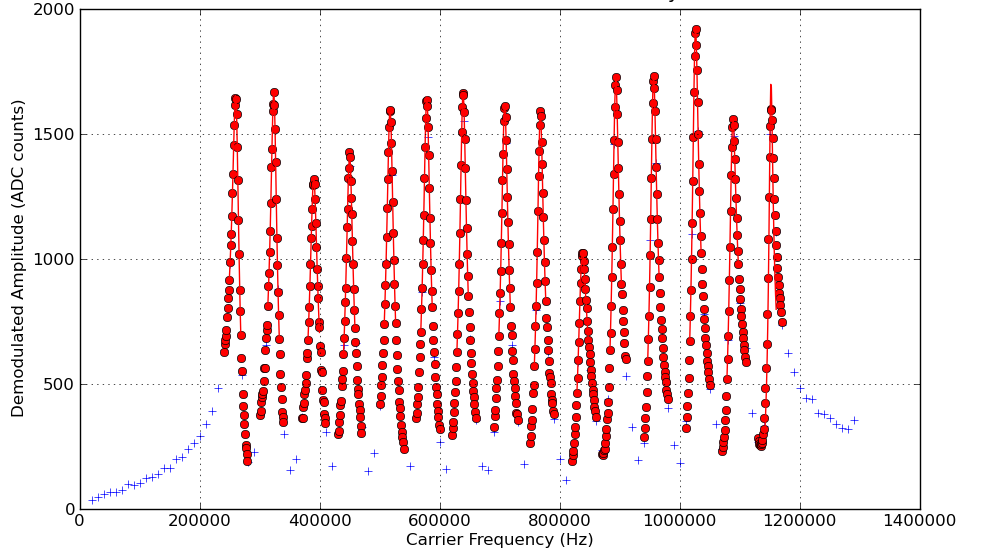
\includegraphics[width=0.98\textwidth]{figures/150-17_SqCh3_netanal_600mK.png}
\caption{A network analysis from wafer 150-17.
\label{fig:network_analysis} }
\end{center}
\end{figure}

Figure~\ref{fig:network_analysis} is a network analysis for a single multiplexed comb of detectors. 
The network analysis swept a voltage across the comb in frequency and measured the current response of the circuit. 
At each LC resonant frequency, the multiplexed RLC circuit peaked in current. 
Around 800~mK, when both the niobium leads and aluminum wirebonds were superconducting, fitting the peak width provided the normal resistance of the \ac{TES}. 
%The shape of the peak was modeled as a Lorentzian, 
%\begin{equation}
%Lorentzian
%\end{equation}
The RLC circuit was modeled to have an impedance of 
\begin{equation}
Z_{RLC_{i}} = ???
\end{equation}
In addition to providing the resonant frequencies, the fit to this model gave the stray resistance and inductance in series with the comb. 
Typical stray resistance was about XXX $\Omega$ and typical stray inductance was XXX $uH$.
Note, the center of the current peak and the optimal frequency bias are not perfectly aligned because we wanted to maximize the current through the bolometer rather than maximize the current through the entire circuit (which included the stray resistance and inductance).

\textcolor{red}{again, I'd like you to remake this figure so the units and axes across figures are consistent ... this one says "f (kHz)", the other says "Carrier Frequency (Hz)"}

\begin{figure}[htbp]
\begin{center}
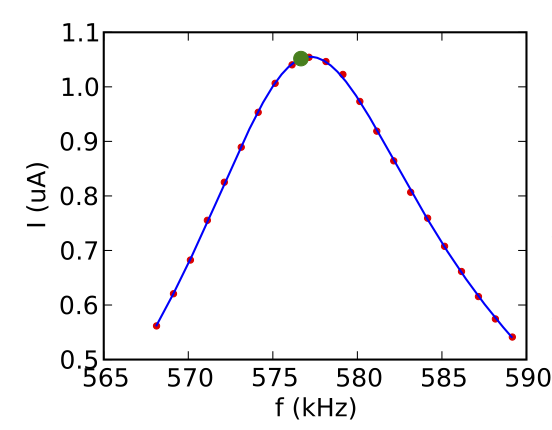
\includegraphics[height=2in]{figures/netanal_zoom.png}
\caption{The fit of a network analysis peak (blue solid) to a Lorentzian and the optimal bias frequency determined (green dot).
\label{fig:network_analysis} }
\end{center}
\end{figure}

\textcolor{red}{Include: Stray impedance measured from an iv curve of a latched/superconducting bolometer.}

Histograms summarizing the measured normal resistance values for the three \ac{EBEX} frequency bands are shown in Fig.~\ref{fig:rn_histograms}. 
%Section~\ref{sec:detector_optimization}. the optimization section doesn't actually provide the detail I want it to provide.
The median normal resistance, $R_{normal}$, for the 150, 250, and 410~GHz bands was 1.9, 1.5, and 1.0~$\Omega$ respectively. 
FROM THE PAPER.
The 150 and 410~GHz bimodal distributions were due to detector parameters being closely grouped within a single fabrication run, but varying between fabrication runs. 
The measured value of $R_{n}$ for the 250~GHz band closely matched the design (see 
Table~\ref{tab:Design_Params}). 
For the other two frequency bands, one mode of the distribution closely matched while the other mode was higher (lower) than design for the 150 (410)~GHz band. 
The 150~GHz detectors with a measured $R_{n}$ of 2~$\Omega$, instead of the nominal 1.5~$\Omega$, were calculated to have increased electrical cross-talk from a value of 0.5\% to 0.9\% and decreased loopgain by 30\%. 
The 410~GHz detectors with a measured $R_{n}$ of 1~$\Omega$, two-thirds of the design value, were calculated to have increased Johnson noise by 20\% relative to the nominal expected value of 4.0 pA$/\sqrt{\mathrm{Hz}}$ (9.4~aW$/\sqrt{\mathrm{Hz}}$); see Equation~\ref{eqn:noisebudget}.

DO YOU WANT TO INCLUDE MORE DETAILS ABOUT THE CROSS-TALK CALCULATION? PROBABLY? 
There is electrical cross-talk between detectors due to the modulation of the detector resistance which results in the modulation of the carrier bias. 
The level of this leakage is approximated by calculating the current modulation due to the neighboring bolometer's carrier bias leaking relative to the on-resonance current modulation for a bolometer. 
\begin{equation}
\frac{R_{bolo}^2}{(2\Delta \omega L)^2}
\end{equation}
~\citep{Dobbs2011}
%see page 100 of notebook for calculation
where for \ac{EBEX} we have inductors $L_{EBEX} = 24~\mu H$ and frequency spacing of at least $\Delta \omega = 2\pi 60~kHz$. 
(The lower bias frequencies have this spacing, but when cooled, the lower capacitance values change more and the resonant frequency spacing is larger than predicted.)
For a detector dropped to 85\% in the transition, having a normal resistance of 1.9~$\Omega$ instead of 1.5~$\Omega$ results in a bias leakage increase of 60\%, increasing the cross-talk from 0.5\% to 0.8\%

%The consequences of overshooting this value, as is the case for many of the 150~GHz detectors, are an increase in the detector voltage bias leakage, which is proportional to $R^2$ \citep{dobbs_revSciInst_2012}, and a decrease in the loopgain, which is inversely proportional to R. 
%% if R is higher, then johnson current noise is decreased since it goes like 1/sqrt(R)
%% if R is higher, then stability requirement has R/(2*pi*L) > 5.8/tau_tes is more satisfied
%For a detector dropped to 85\% in the transition, having a normal resistance of 1.9~$\Omega$ instead of 1.5~$\Omega$ results in a bias leakage increase of 60\%, increasing the cross-talk from 0.5\% to 0.8\%, and a loopgain decrease of 30\%. 
%The consequence of undershooting the normal resistance, as is the case for many of the detectors on wafer 410-28, is an increase in the Johnson current noise. The Johnson noise is proportional to $1/\sqrt{R}$, so that noise term increases by 20\% given a value of 1.0~$\Omega$ instead of 1.5~$\Omega$.



%\comred{Assume detector optimization explains what about the electronics set our target to be 1.5~$\Omega$? Ben says "The requirement is really ~1.25 because what actually matters is Rtes in transition for the L/R requirement.  So depending on how deep we get in to the transition we could start anywhere just above 1.2 Ohms to operate at 0.88 to 1.0 Ohms." BUT. When determining which Rfrac to tune to, we didn't do this calculation. Rather, we noted, in general, below 80\% $R_{start}$, we had (not well understood) excess noise and so opted to go to 85\%. What I'm trying to say is, in practice, the operating fracRn value was not chosen carefully on a bolo by bolo basis or even a wafer by wafer basis to achieve a specific L/R. Explain the consequence of having a higher or lower normal resistance, e.g. 150s and one of the 410s (was it the 410 that operated or the 410 that was saturated?)? Ben says "Increased johnson noise and possibly bolo stability.  However, I'm not sure if either of these effects were detected in the wafers in test cryostats, Palestine, or flight."}


\begin{figure}[ht!]
\centering
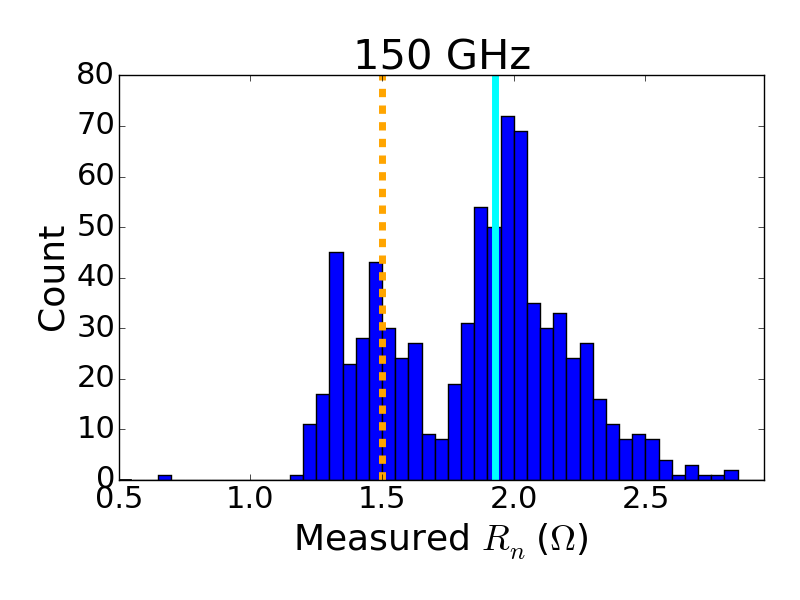
\includegraphics[width=0.31\textwidth]{figures/150_rn_hist.png}
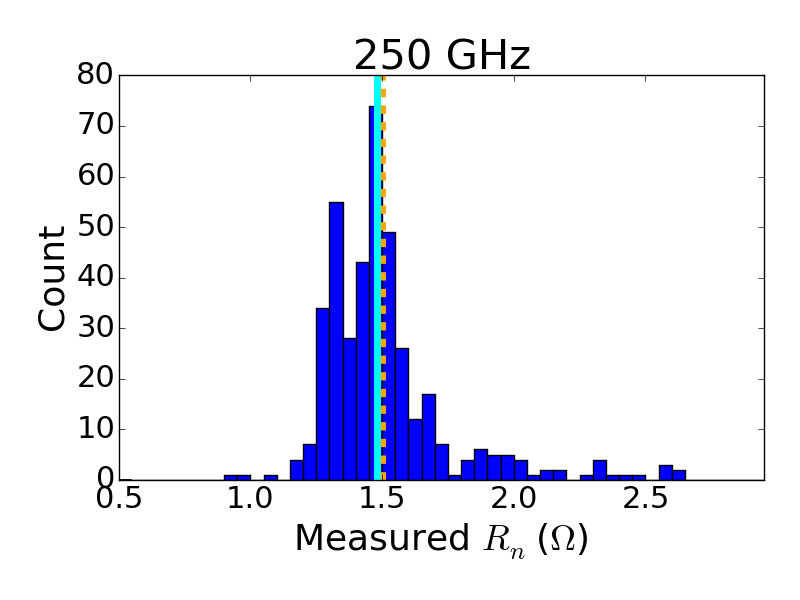
\includegraphics[width=0.31\textwidth]{figures/250_rn_hist.png}
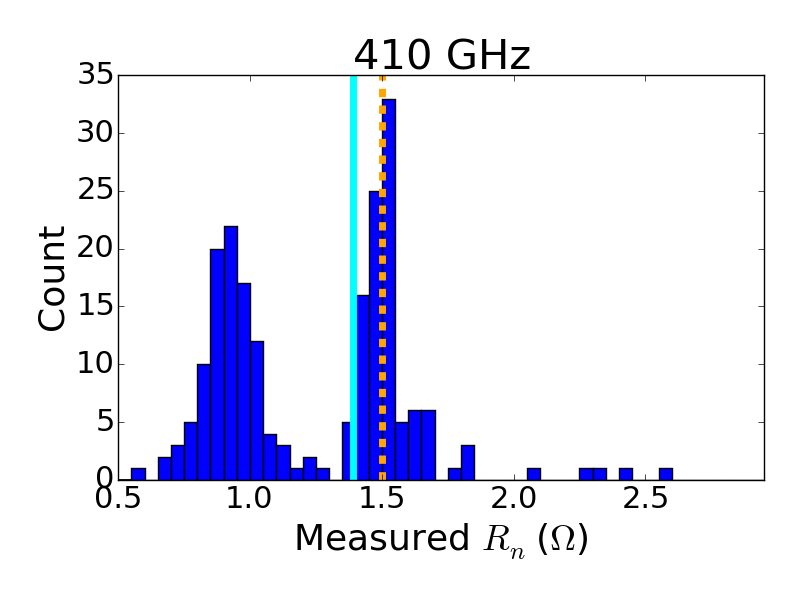
\includegraphics[width=0.31\textwidth]{figures/410_rn_hist.png}
\caption{Histogram of measured normal resistances $R_{n}$ for each of the frequency bands, including the median (vertical cyan)  
and design (vertical gold dashed) values.
}
\label{fig:rn_histograms}
\end{figure}

%%%%%%%%%%%%%%%%%%%%%%%%%%%%%%%%%%%%%%%%%%%%%%%%%%%%%%%%%%%%%%%%%%%%%%%%%%%%%%%%
\subsection{Critical Temperature}
\label{sec:critical_temp}
%TOWARDS CRITICAL TEMPERATURES
%%%%%%%%%%%%%%%%%%%%%%%%%%%%%%%%%%%%%%%%%%%%%%%%%%%%%%%%%%%%%%%%%%%%%%%%%%%%%%%%

(HAVE WE MOTIVATED ELSEWHERE WHY WE CARE ABOUT VALUE OF $T_{C}$?) 
For the measurement of the critical temperature, we placed a voltage bias of 5~$nV_{rms}$ across the detector such that the Joule heating was negligible ($\frac{V^2}{R} = 1.5~fW$) but there was still a measurable current signal. 
Then we slowly, usually less than 3~mK/min, both cooled and warmed the detectors through their transitions while measuring the current through the detector. 
We converted to resistance using Ohm's law, $R=V_{bias}/I_{measured}$.
Note, this resistance does not agree with the resistance measured via the network analyses or via the IV curves. Any ideas why?

Fig.~\ref{fig:tc_measurement} is an example of a critical temperature measurement for one detector. 
The top panel shows the detector temperature as a function of time. %no need to point out there is hysteresis inherent in this measurement because the temperature sensor is on the invar, not on the wafer? 
The bottom two panels show the bolometer resistance as a function of time and temperature. 
The hysteresis between the critical temperature measured cooling and warming is generally less than 5~mK, sufficiently accurate for characterization.

\begin{figure}[htbp]
\begin{center}
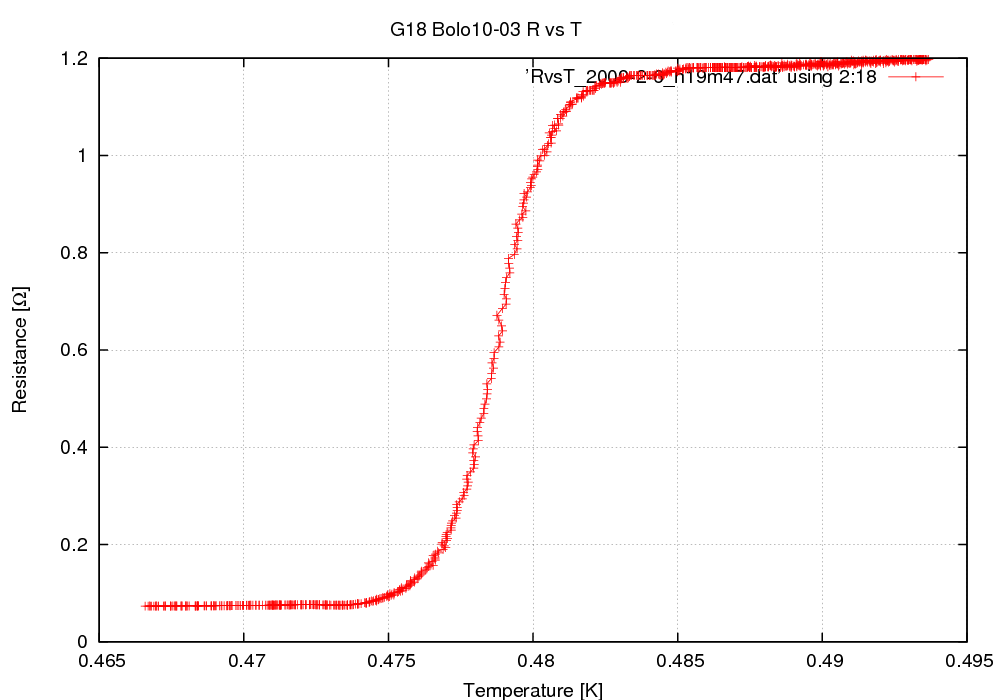
\includegraphics[height=2.5in]{figures/G18_bolo10-03_RvsT_oral}
\caption{FIND/MAKE THIS FIGURE: WANT WARMING AND COOLING IN ETC. BE CLEAR ABOUT HYSTERESIS FROM WARMING AND COOLING. NOTE LAG DUE TO TEMPERATURE SENSOR BEING MOUNTED TO INVAR INSTEAD OF TES.
\label{fig:tc_measurement} }
\end{center}
\end{figure} 

Histograms summarizing the measured critical temperatures for the three \ac{EBEX} frequency bands are shown in Fig.~\ref{fig:tc_histograms}. 
The target critical temperature for each band is 0.44~K, a value which optimizes the phonon noise term given the \ac{EBEX} bath temperature. %or refer to Section~\ref{sec:detector_optimization} for the motivation ??
We find the median critical temperature for the 150, 250, and 410 GHz bands to be 0.45, 0.49, and 0.51~K respectively.  
The consequence of overshooting the critical temperature, as for some of the detectors in each of the frequency bands, is an increase in the Johnson noise, proportional to $\sqrt{T}$, and an increase in the phonon noise, proportional to $T$. 
The consequence of undershooting the critical temperature, as for roughly half of the 150~GHz detectors, is potentially not being able to drop the detector into the transition because the critical temperature is too close to the bath temperature. % is this actually why we didn't want to go too low?
%\comred{what's the consequence of the wide spread in Tc for the 150s? how concerned are we about the level of spread we fabricated?}

FROM THE PAPER.
For the measurement of the critical temperature $T_{c}$ we biased the detectors with 5~nV such that the Joule heating of 1.5~fW was 
small and the bath temperature was a good proxy for the bolometer's temperature. For the same reason, the measurement was 
done in dark conditions. We slowly changed the detectors' temperature while monitoring their current. 
At the critical temperature the current showed a steep transition.
Figure~\ref{fig:tc_histograms} shows histograms summarizing the measured critical temperatures. There 
was a $\sim$20\% wafer-to-wafer spread in the measured $T_{c}$ with the medians for the three bands within 
16\% of the target value of 0.44~K. 
The 150~GHz detectors have the widest spread of measured $T_{c}$. The effect of this spread is to increase Johnson (phonon) 
noise when $T_{c}$ is above (below) the design value. 
At the high (low) edge of the distribution with $T_{c}$~=~0.54~K (0.36~K), there was an 11\% (5\%) increase in the calculated Johnson (phonon) noise 
relative to the nominal expected value of 4.0~pA/$\sqrt{\mathrm{Hz}}$ (20~aW/$\sqrt{\mathrm{Hz}}$). 



\begin{figure}[ht!]
\centering
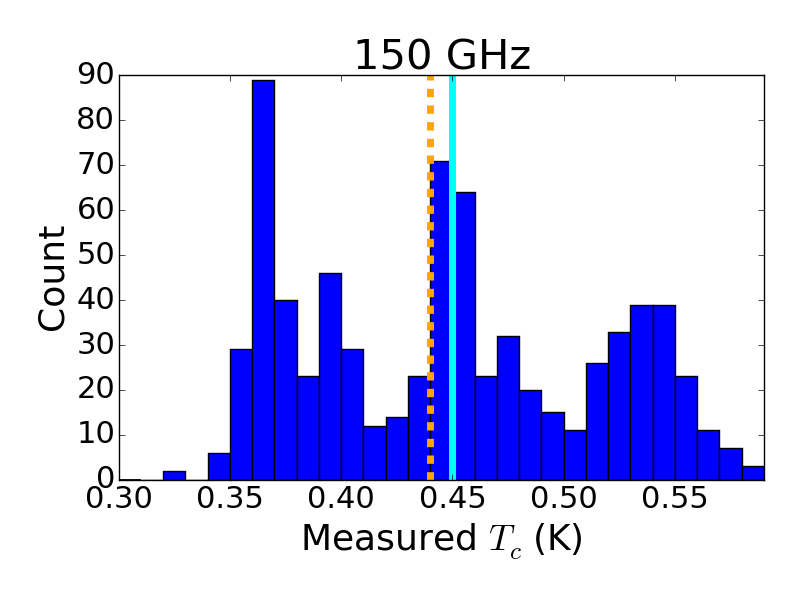
\includegraphics[width=0.31\textwidth]{figures/150_tc_hist.png}
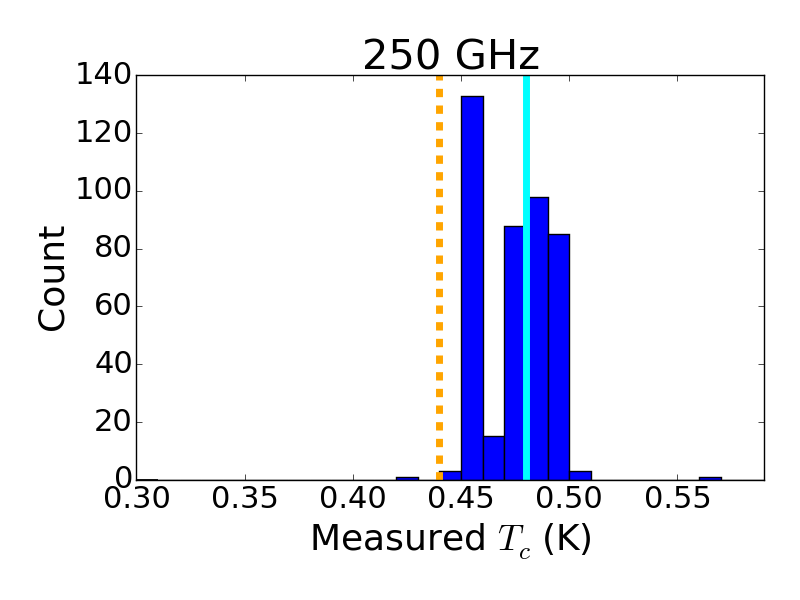
\includegraphics[width=0.31\textwidth]{figures/250_tc_hist.png}
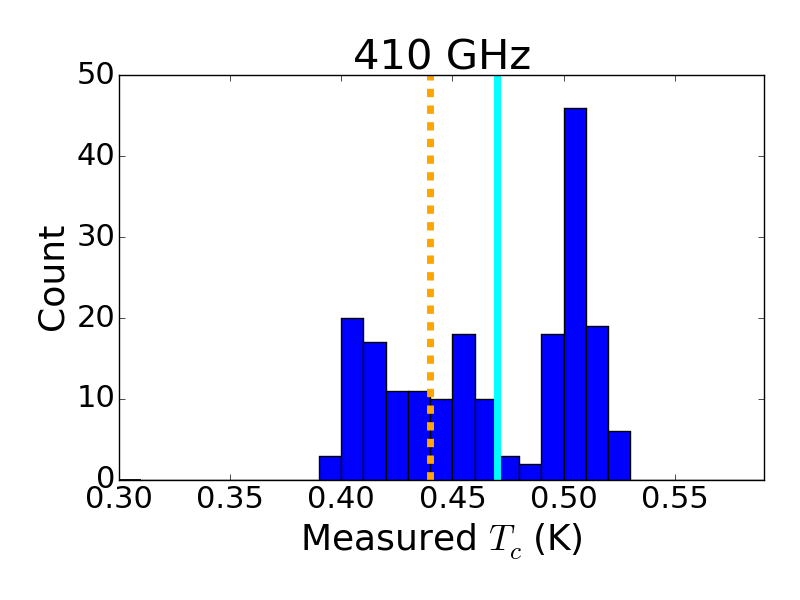
\includegraphics[width=0.31\textwidth]{figures/410_tc_hist.png}
\caption{Histogram of measured critical temperature values for the detectors in each frequency band including the median (vertical cyan) and design (vertical gold dashed) values. 
\label{fig:tc_histograms} }
\end{figure}

%%%%%%%%%%%%%%%%%%%%%%%%%%%%%%%%%%%%%%%%%%%%%%%%%%%%%%%%%%%%%%%%%%%%%%%%%%%%%%%%
\subsection{Thermal Conductance}
\label{sec:thermal_conductance}
%TOWARDS THERMAL CONDUCTANCES 
%%%%%%%%%%%%%%%%%%%%%%%%%%%%%%%%%%%%%%%%%%%%%%%%%%%%%%%%%%%%%%%%%%%%%%%%%%%%%%%%

\textcolor{red}{will you have already discussed \ac{NEP}? Yes. In 2.1. Bolometer Theory. in particular, phonon noise. for now point to eqtn in measured noise section.}

\textcolor{red}{you need to be clear that you are using noise and \ac{NEP} interchangeably.}

\textcolor{red}{Address: Why do we need to know the thermal conductance? i.e. Why do we care? When we talked about targets, we already should have talked about including a safety factor? And what set that target? maybe all of these words need to be moved to the bolometer theory section?}
% too vague. The thermal conductance of the thermal link from the TES to the bath governs the bolometer sensitivity. 

\textcolor{red}{Doesn't it make sense to expand on the sources of radiative load? and instead of saying expected load, say exactly what the expected load was?}

\textcolor{red}{ What happened when we measured $P_{elec}$ in ebex vs etc vs mcgill? How do we deal with different bath temperatures?}

\textcolor{red}{What have we learned from the thermal conductance measurements? How did we (attempt to) modify detector fabrication given our measurements?}

\textcolor{red}{You need to say what bath temperature these average thermal conductances are quoted at and how you got them.}

\textcolor{red}{How do we measure the thermal conductance? (Be sure you explain how we get from IV to PV and how we extract $P_{electrical}$ and how wrong we might be about this number.)}

\textcolor{red}{Talk about dropping one bolometer at a time versus dropping the entire comb? i.e. talk about cross-talk? and how it's more dramatic when overbiased because the signal you're supplying is stronger?}

\textcolor{red}{Talk about why it's not correct to do the ratio of vbias/imeasured and call that R? what uncertainty does this introduce?}

\textcolor{red}{Talk about the stray impedance effect you modeled. also, trevor lanting talked about this? in the case of a well-behaved bolometer with small stray impedance, \cite{lanting_thesis} \textcolor{red}{fix citation}}

\textcolor{red}{In bolometer theory, you need to have already explained electrothermal feedback.}

\textcolor{red}{Discuss results. What are the major uncertainties in this measurement? Talk about how deep you drop and how you define depth in transition. (will address noise as function of depth in transition in dark noise section).}

\textcolor{red}{Do you want to include double transition iv curve? e.g. /data/ebex3/systems/nigel/data/2010/nigel.backup.data/07/30/boloIV.340mK/plots/250-01-02.IV.201007301208.png}


\textcolor{red}{are you going to comment on how the resistance measured for this bolo (2.9 $\Omega$) compares to the resistance measured via the network analysis? put that information in a loopgain section instead?.}

\textcolor{red}{are you going to comment on WHY the fit gives a non-zero current offset?}

\textcolor{red}{You need to talk about going from average thermal conductance to dynamic thermal conductance ... does that belong here? no, I think it'd be better in bolometer theory or in the measured noise section. and it'll be fine if you also move the top paragraph out.}

 \textcolor{red}{I wish you could find or rewrite the code to make the bolo.iv.curve figures - the pW are in square brackets and all the others in parenthesis. and the axis labels are smaller than I want them to be.}


\textcolor{red}{Use this R vs V curve to help explain how deep in the transition the detectors are dropped. point out why it isn't the greatest way. Also, point out that R at high values of $V_{bias}$ still has some slope (how much slope?), so it's not obvious where to define $R_{normal}$. }

\textcolor{red}{You need to comment on the $\overline{G}$ distribution shapes and consequences of overshooting, e.g. for 410~GHz.}

\textcolor{red}{Mention voltage bias is kind of a proxy for temperature? i.e. R vs V is effectively an R vs T curve where we don't have a calibration for the x-axis?}

The detector sensitivity is a function of the thermal conductance, $G$, of the link from the TES to the bath. %, Figure~\ref{fig:bolometer_cartoon}.
In particular, the phonon \ac{NEP} is proportional to $G$, Equation~\ref{eq:nep}. 
We want to minimize $G$ so that we minimize the detector \ac{NEP} and thus maximize the detector sensitivity. 
This value of $G$, however, needs to be sufficiently high to allow for the detectors to operate in the presence of the radiative load at float, Section~\ref{sec:detector_design}. 
%as well as any fluctuations in load %fluctuations are a problem for ground-based expt's, not us
The dark test cryostat measurements of $G$ allowed us to predict the phonon \ac{NEP} for each detector and also determine if there would be sufficient dynamic range to operate the detectors under the expected loading conditions. 

In practice, we measured the average thermal conductance, $\overline G$, as opposed to the dynamic thermal conductance, $G$.
Then, knowing the bath temperature, the bolometer temperature, and the power of thermal conductivity, we used \textcolor{red}{EquationThatDoesn'tExistYet} to relate our measurement of $\overline G$ to $G$. 
In order to measure $\overline G$, we performed an IV curve for each bolometer.
That is, we stepped down the voltage bias, typically in steps of 0.05~$\mu V$, and measured the current through the bolometer. 
At each step, the instantaneous resistance, the ratio of the voltage bias to the current measured, was calculated, Figure~\ref{fig:bolo_rv_curve}. 
The bias voltage of each bolometer was dropped until the ratio of the voltage bias to the current measured reached a fixed fraction of its original value.
In the test cryostats, the fraction was typically 0.7. 
For \ac{EBEX2013}, the fraction was 0.85 for the majority of flight.
The value used in flight was higher than the nominal lab value because in the test cryostats the bolometer noise performance deeper in the transition diverged from the predictions, Section~\ref{sec:dark_noise}. 
%Note, in Figure~\ref{fig:bolo_rv_curve}, in the over-biased, normal region, the resistance of the bolometer has a non-zero slope. 

\begin{figure}[htbp]
\begin{center}
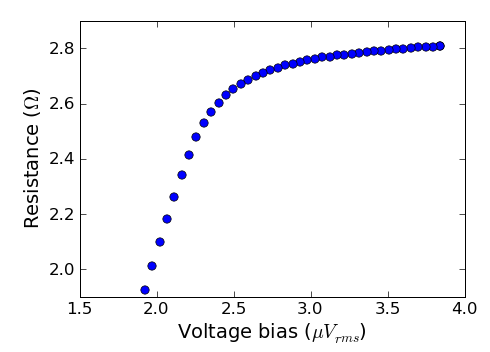
\includegraphics[height=2in]{figures/RV_201007301208.png} 
\caption{The instantaneous resistance ($I \over V$) of a 150-01 bolometer as a function of the voltage bias across the bolometer. This bolometer was dropped to 0.7 of the starting value. 
\label{fig:bolo_rv_curve} }
\end{center}
\end{figure}


Example IV and PV curves from one detector on wafer 150-01 are shown in Figure~\ref{fig:bolo_iv_curve}.
Above the superconducting transition, at higher voltage biases, the AlTi bilayer of the \ac{TES} was normal and so the current was proportional to $1 / R$. 
Fitting the normal region for this particular detector gave a resistance of 2.9 $\Omega$. 
As the bilayer began to superconduct, the resistance dropped and the current measured turned around with a characteristic smooth checkmark shape. 
Once the bolometer was sufficiently far into the superconducting transition, electro-thermal feedback caused the power dissipated in the bolometer to remain fixed, Section~\ref{sec:tes_bolometer}.
When we plot the power dissipated in the bolometer ($I \times V$), the electrical power required to hold the detector in the transition is the horizontal section of the PV curve.

\begin{figure}[htbp]
\begin{center}
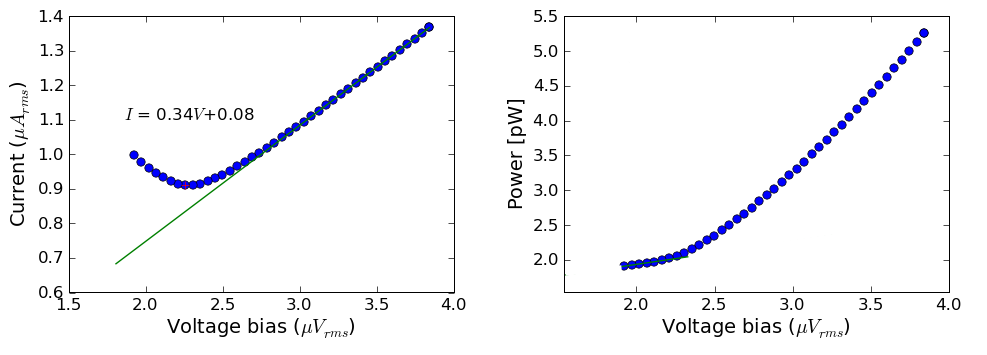
\includegraphics[width=0.99\columnwidth]{figures/IV_201007301208.png} 
\caption{Left: The current through the \ac{SQUID} as function of the voltage bias across the bolometer. Right: The electrical power dissipated in the bolometer ($I / V$) as a function of the voltage bias across the bolometer.
\label{fig:bolo_iv_curve} }
\end{center}
\end{figure}

%As the Joule Power decreases, the detector temperature decreases towards its transition temperature and the . 

Because each bolometer wafer is enclosed in a light-tight box for the dark characterization tests, there is negligible radiative power and so the total electrical power measured from the PV curve is the total power dissipated in the detector. 
This power is often referred to as the saturation power, $P_{sat}$. 
The detector in Figure~\ref{fig:bolo_iv_curve} has $P_{sat} = 1.9~pW$.
Though $P_{sat}$ is just $G$ with the bath and bolometer temperatures folded in, it can be a useful parameter to think in terms of because the bolometer loses nearly all sensitivity if it saturates, i.e. if $P_{sat}$ is less than the radiative load during observations. 
%the sensitivity of the bolometer increases with lower saturation power (lower $G$), but 

The average thermal conductance of the weak link was calculated from the saturation power, measured from the PV curve, and the critical temperature, Section~\ref{sec:critical_temp}, 
\begin{equation}
\overline{G}(T_{bath}) = \frac{P_{sat}(T_{bath})}{T_{c} - T_{bath}}
\end{equation}
Histograms summarizing the measured average thermal conductance values for the three \ac{EBEX} frequency bands are shown in Figure~\ref{fig:G_Histograms}.
We found the median average thermal conductance, $\overline{G}$, for the 150, 250, and 410 GHz bands to be 36, 51, and 69~pW/K respectively. 
The target values for the average thermal conductances were set by the radiative loading in the balloon environment, Section~\ref{sec:detector_optimization}, and were 30, 40, and 50~$pW/K$ for the 150, 250, and 410~GHz bands respectively. 
The goal was to err on the higher side of the target and take the hit in phonon noise rather than risk rendering the detectors inoperable because of too little thermal conductance for the radiative load. 

\begin{figure}[ht!]
\centering
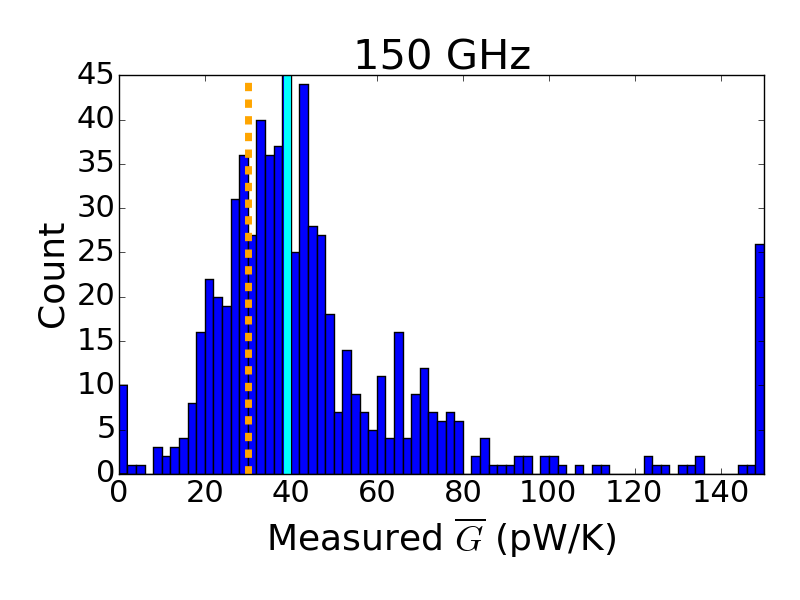
\includegraphics[width=0.32\columnwidth]{figures/150_g_bar_hist.png}
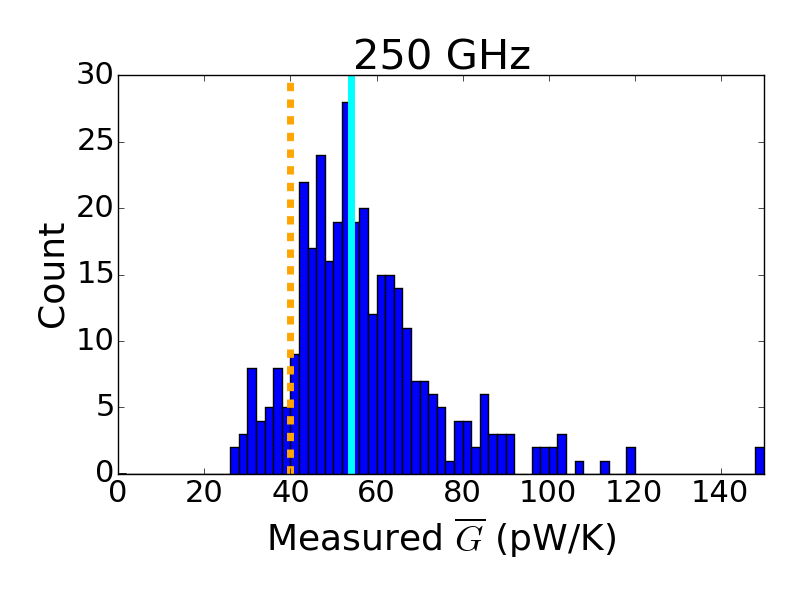
\includegraphics[width=0.32\columnwidth]{figures/250_g_bar_hist.png}
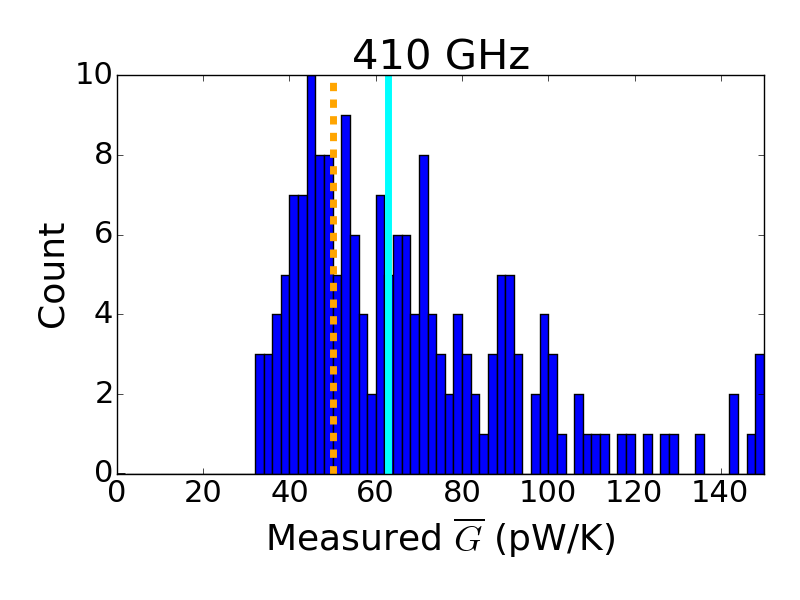
\includegraphics[width=0.32\columnwidth]{figures/410_g_bar_hist.png}
\caption{Histograms of the measured average thermal conductance values for the three frequency bands including the 
median (vertical cyan) and design (vertical gold dashed) values. 
We piled measurements of  $\overline{G}$ exceeding 150~pW/K into the last histogram bin.
}
\label{fig:G_Histograms} 
\end{figure}



%\textcolor{red}{This doesn't matter? You're not giving a play-by-play accounting.}
%Once the resonant frequencies are determined from the network analysis fits, the stage is heated so the bolometers are above their critical temperatures. 
%The bolometers are then electrically overbiased such that there is enough Joule Power dissipated in the \ac{TES} to keep its resistance normal as the stage is cooled. 
%Once the stage is at its base temperature, we measure the bolometer saturation powers. 


FROM THE PAPER
We determine the average thermal conductance of the bolometers using the relation
\begin{equation}
 \overline{G}(T_{0}) = P_{sat}(T_0)/ (T_{c} - T_{0}),
\label{eqn:gbar}
\end{equation}
where $P_{sat}$ is the total power deposited in the detector, which is the power necessary to operate the \ac{TES} in the regime of strong electrothermal feedback in which the total power absorbed is constant.
This power is commonly called the `saturation power' and it depends on the temperature of the bath
\begin{equation}
P_{sat}(T_{0}) = P_{e} (T_{0}) + P_{abs}. 
\label{eqn:boloPowerFlow}
\end{equation}
Here $P_{e}$ is the electrical power absorbed in Joule heating and $P_{abs}$ is the radiative power absorbed.
In dark conditions we assume that $P_{abs}$~=~0, and so $P_{sat}(T_{0})$~=~$P_{e,d}(T_{0})$ is 
therefore a measurable quantity; we added the subscript $_{d}$ to $P_{e,d}$ to highlight that this is the electrical 
power measured in dark conditions. 

FROM THE PAPER
Histograms summarizing the measured average thermal conductance values for the three \ac{EBEX} frequency bands are shown in 
Figure~\ref{fig:G_Histograms}. The values of  $\overline{G}$ are given for the \ac{EBEX} bath temperature, $T_{0}$~=~0.25~K.
The measurements were conducted in three different cryostats, each operating at 
a different bath temperature $T_{0'}$. We corrected the measured values $\overline{G}(T_{0'})$ to $\overline{G}(T_{0})$ using 
the scaling
\begin{equation}
P_{sat}(T_0) = \left( \frac{T^{n+1}-T_0^{n+1}}{T^{n+1}-T_{0'}^{n+1}} \right) P_{sat}(T_{0'}),
\label{eqn:ScalePsat}
\end{equation}
which assumes that the thermal conductivity follows a power law $\kappa$~=~$\kappa_{0} T^{n}$; see Section~\ref{sec:optical_time_constant}. 

FROM THE PAPER
The design and median of measured values for the average thermal conductances are given in Table~\ref{tab:Design_Params}. While the 
measured medians are up to 40\% larger than the design values, the spread in the measurements is even larger. This spread is 
a consequence of variance between wafers and is also apparent in the measurements of $T_{c}$. 
Higher thermal conductance increases phonon noise. For example, for a median 410~GHz detector, phonon noise increased by 
% for histograms using only flight bolos, median was 69
%17\% relative to the nominal value of 26~$aW/\sqrt{Hz}$.
% for histograms using all ground characterization data, median is 63. so percent decreased. 
12\% relative to the nominal value of 26~$aW/\sqrt{\mathrm{Hz}}$. 


%%%%%%%%%%%%%%%%%%%%%%%%%%%%%%%%%%%%%%%%%%%%%%%%%%%%%%%%%%%%%%%%%%%%%%%%%%%%%%%%
\subsection{Optical Efficiency}
\label{sec:optical_efficiency}
%%%%%%%%%%%%%%%%%%%%%%%%%%%%%%%%%%%%%%%%%%%%%%%%%%%%%%%%%%%%%%%%%%%%%%%%%%%%%%%%

\begin{figure}[ht!]
\begin{center}
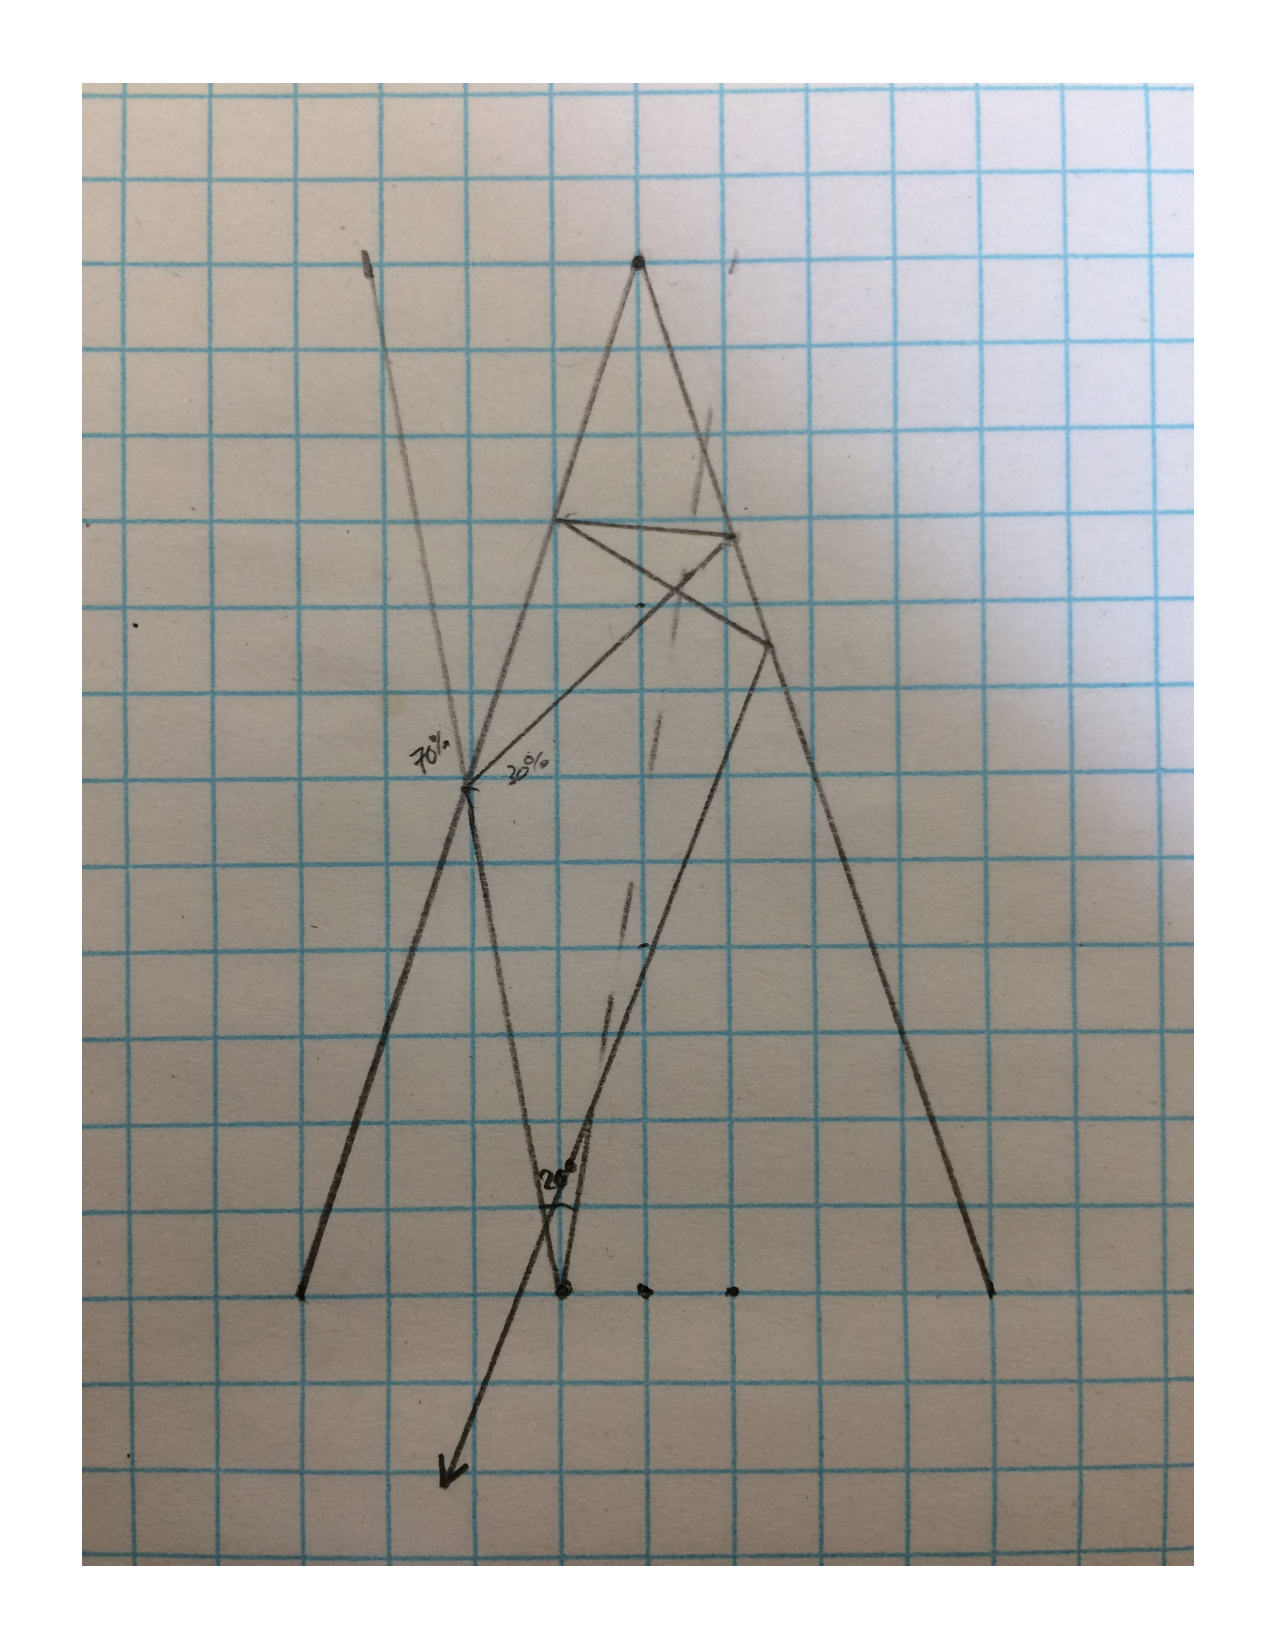
\includegraphics[height=2.5in]{figures/blackbody_design2}
\caption{Eccosorb blackbody design. 
\label{fig:blackbody_design} }
\end{center}
\end{figure}

\begin{figure}[ht!]
\begin{center}
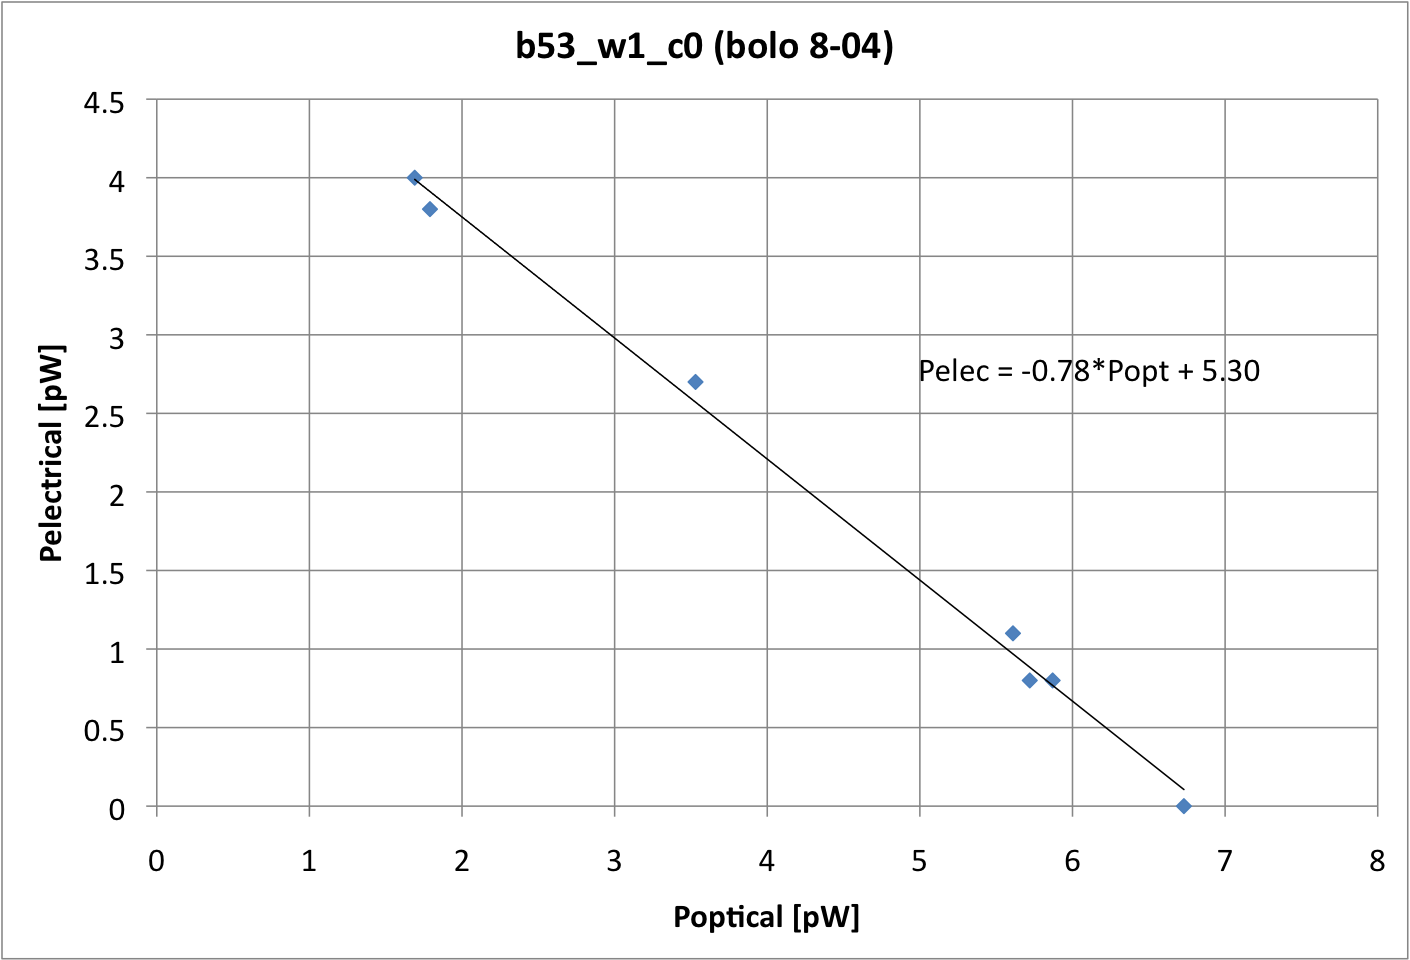
\includegraphics[height=2.5in]{figures/Nb01_PelecvsPopt_b53_w1_c0}
\caption{One 150-01 detector electrical power as function of blackbody power. The slope is the detector's optical efficiency. 
\label{fig:pelec_vs_popt} }
\end{center}
\end{figure}


\begin{figure}[ht!]
\begin{center}
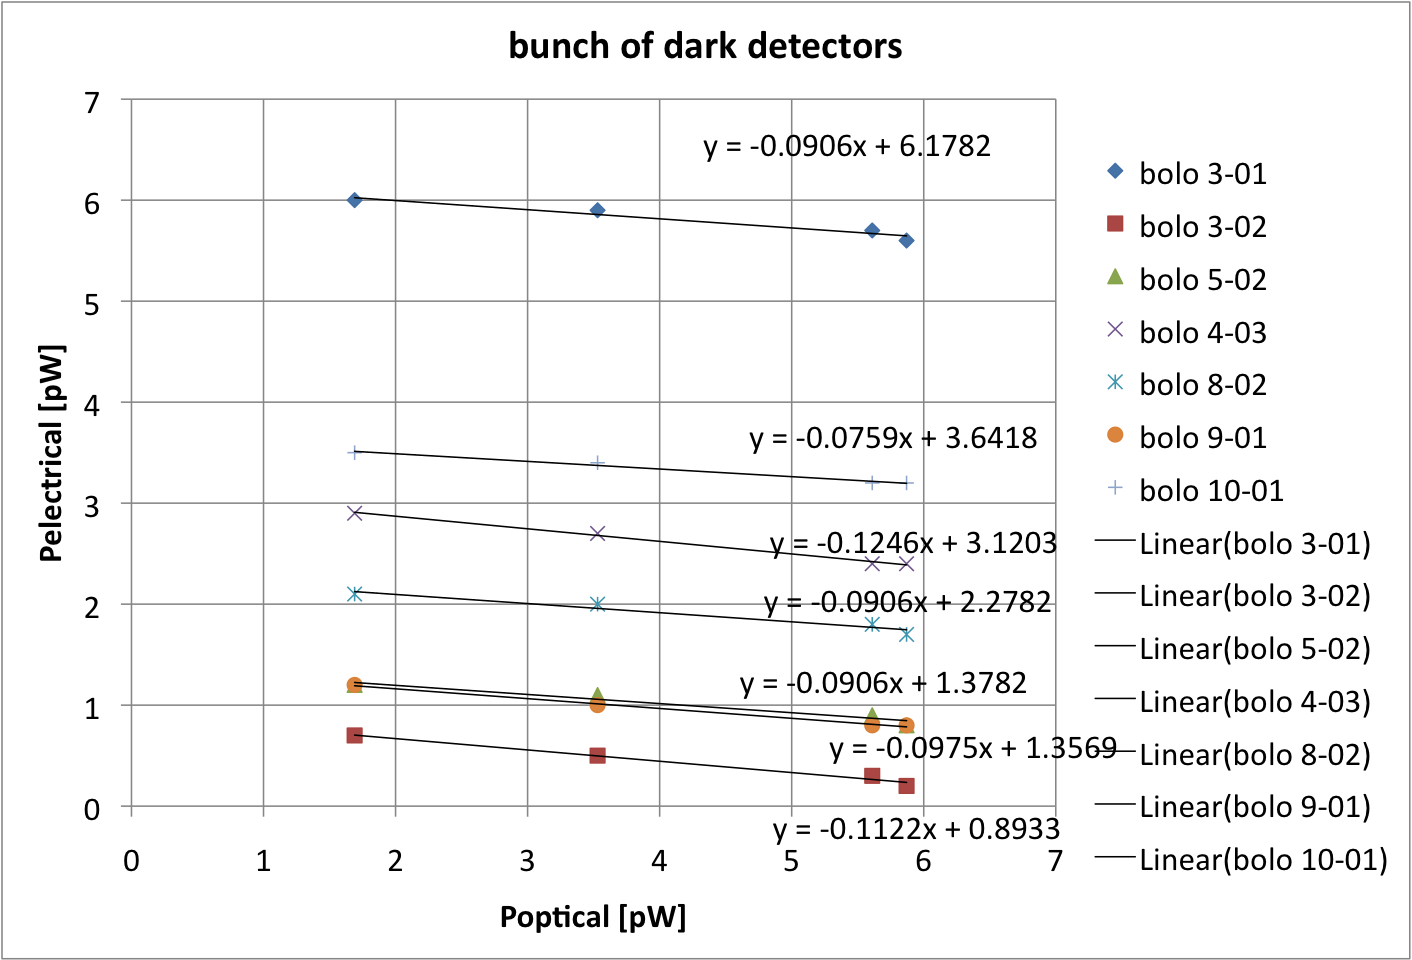
\includegraphics[height=2.5in]{figures/darkdetectoreffs}
\caption{The dark detectors also observed a decrease in electrical power needed to keep the detector in the transition as the black body temperature was turned up. The slope of this line gives the "efficiency" of the dark detectors. Some measure of the level of optical cross talk?
\label{fig:dark_optical_efficiencies} }
\end{center}
\end{figure}


%%%%%%%%%%%%%%%%%%%%%%%%%%%%%%%%%%%%%%%%%%%%%%%%%%%%%%%%%%%%%%%%%%%%%%%%%%%%%}}}

%%%%%%%%%%%%%%%%%%%%%%%%%%%%%%%%%%%%%%%%%%%%%%%%%%%%%%%%%%%%%%%%%%%%%%%%%%%%%%%%
\subsection{Time Constants}
\label{sec:time_constants}
%%%%%%%%%%%%%%%%%%%%%%%%%%%%%%%%%%%%%%%%%%%%%%%%%%%%%%%%%%%%%%%%%%%%%%%%%%%%%%%%

\textcolor{red}{Does this section get to make it in? We have electrothermal taus and IR taus ... Karl's fits were much more sophisticated. Can I include my stupid "fits"?}

\begin{figure}[ht!]
\begin{center}
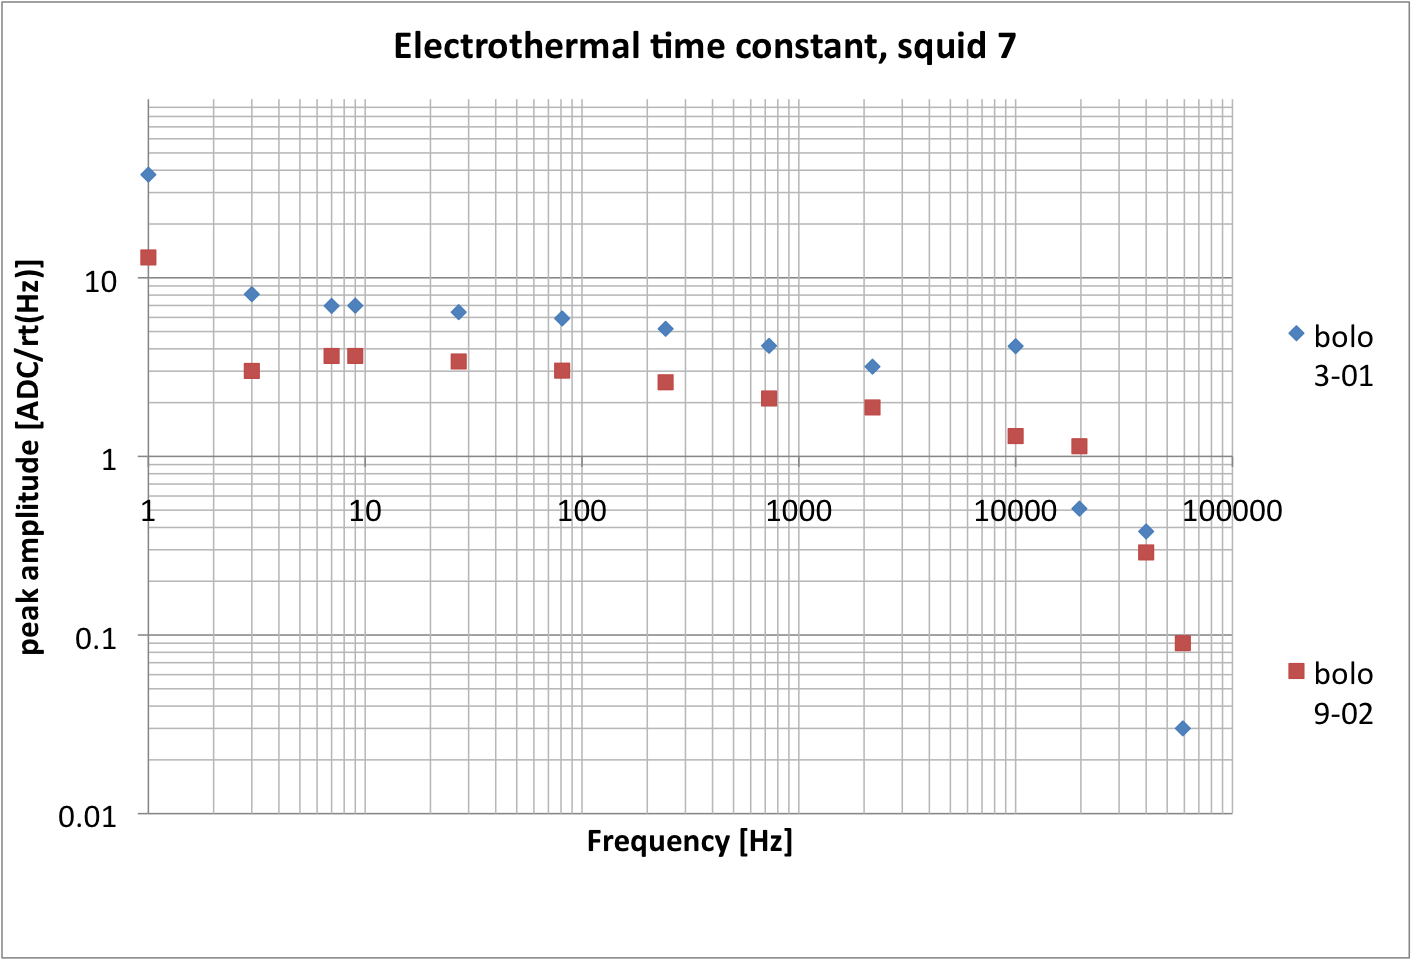
\includegraphics[height=2.5in]{figures/Nb01_squid7_etau_morepts}
\caption{Electrothermal time constants of two bolometers on 150-01. What does the fit to this data give? This is the time constant between the TES and the web? As expected, the for the web to thermalize is much faster than the optical time constant (time for light to couple to the web). 
\label{fig:electrothermal_tau} }
\end{center}
\end{figure}


%%%%%%%%%%%%%%%%%%%%%%%%%%%%%%%%%%%%%%%%%%%%%%%%%%%%%%%%%%%%%%%%%%%%%%%%%%%%%}}}



%%%%%%%%%%%%%%%%%%%%%%%%%%%%%%%%%%%%%%%%%%%%%%%%%%%%%%%%%%%%%%%%%%%%%%%%%%%%%%%%
% Dark Noise Performance {{{
%%%%%%%%%%%%%%%%%%%%%%%%%%%%%%%%%%%%%%%%%%%%%%%%%%%%%%%%%%%%%%%%%%%%%%%%%%%%%%%%
\section{Dark Noise Performance}
\label{sec:dark_noise}
%%%%%%%%%%%%%%%%%%%%%%%%%%%%%%%%%%%%%%%%%%%%%%%%%%%%%%%%%%%%%%%%%%%%%%%%%%%%%%%%

The noise measurements were broken down in order to determine if the performance of each part of the detector readout chain was as expected. 
That is, we measured the warm electronic noise open loop (with the squids off), the electronic noise up to and including the squids (with their feedback loops closed), the noise of resistor channels (i.e. the entire electronic chain up to the bond pads on the \ac{LC} board), the noise of the bolometers over-biased with the stage above the bolometers' $T_{c}$, the noise of the bolometers overbiased with the stage at the refrigerator's base temperature, and the noise of the bolometers in-transition as a function of their transition depth. 



\textcolor{red}{can you draw a circuit diagram of the warm electronic noise you're measuring?}

\textcolor{red}{Which electronic component is responsible for the roll off? It is the squid controller first stage amplifier. Can you get the specs to determine what roll off we expected? Can't find on wiki. Ask Franky. Then, answer, is it consistent with what we measured?}

\textcolor{red}{do you understand why we don't have this roll off when it's operating under normal conditions and why we DO have this roll off when it's open loop?}

\textcolor{red}{Is this $V_{rms}$ or $V_{p}$ ?}

\textcolor{red}{As you talk about noise, you need to be clear somewhere that you're using NEP and noise and ASD and PSD interchangeably. OR. don't use them interchangeably!}

\textcolor{red}{Are you sure you have the contribution calculations correct? What are those $\sqrt{2}$s coming from??}

\textcolor{red}{If you're going to mention the 20 ohm resistor noise as a main contributor, you need to be able to point to where this is. perhaps say it in words and refer to Franky's thesis??}

\textcolor{red}{before you dive in to plots where you have the white noise level/asd plotted on the y-axis, you need to describe how you obtained those data points!}

\textcolor{red}{Can you please be more specific about exactly which electronic components are included in this measurement?}

\textcolor{red}{Is there an apparent paradox here? You are measuring the warm electronic noise with the squids off, open loop. and you say the largest contributors are the 1st stage amplifier and the 20 ohm resistor. AND, you say those two noise contributions are the only reason you need the squid transimpedance. you're missing a key connection... when you close the feedback loop, then dv/di matters??? and when it's open, the noise prediction changes??}

\textcolor{red}{It's confusing to say the squids are off and then to say you've measured the noise for two squids ... word this better if you have time!}


With the \ac{SQUID}s off, we measured the open loop noise.
%(no current bias, no flux bias, and no voltage offset) % no need to define off ... also, that's the voltage offset of ... the firs stage amplifier???
This was a measure of the noise of the warm electronics up to the \ac{SQUID} controller first stage amplifier. 
The theoretical open loop transfer function was 0.774 nV to 1 \ac{ADC} count. 
The measured transfer function was a factor of 1.13 greater than the theoretical. 
Figure~\ref{fig:dark_electronic_noise} is the measured open loop warm electronics noise for two \ac{SQUID}s in \ac{ETC} as a function of the demodulation frequency. 
The total noise prediction was $1.33~nV/\sqrt{Hz}$, determined from the electronic specifications~\ref{frankys_thesis}. 
The largest contributors were the first stage amplifier of the \ac{SQUID} controller board, $0.85~nV/\sqrt{Hz}$, and that amplifier's $20~\Omega$ gain defining resistor Johnson noise, $0.57~nV/\sqrt{Hz}$. 
The measurement agrees with the prediction at low frequencies and then the signal rolls off, with a -3dB point around 1~MHz, because the first stage amplifier is being operated in the open-loop regime~\ref{data_sheet?}.  

\begin{figure}[ht!]
\begin{center}
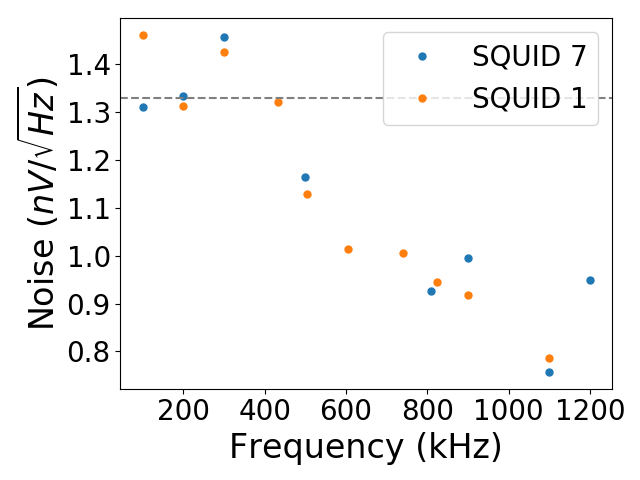
\includegraphics[height=2.5in]{figures/warm_electronic_noise.png}
\caption{Measured noise of the warm electronics in \ac{ETC} up to the first stage amplifier on the \ac{SQUID} controller board. The open loop noise at low frequencies was predicted to be 1.33~$nV/\sqrt{Hz}$ and to roll off with a -3dB point around 1~MHz. 
\label{fig:dark_electronic_noise} }
\end{center}
\end{figure}


\textcolor{red}{Are you at all interested in recording, for posterity's sake?, how you converted from $V_{DAC}$ to physical units?? i.e. for the \ac{ETC} \ac{SQUID} controller board, $1 V_{DAC} = 1 mV$ and $1 V_{DAC} = 20 \mu A$ and mention mutual inductance $\phi_{0}/26 \mu A$?}

\textcolor{red}{do you want to mention what transimpedances we measured with the ebex squids?}

\textcolor{red}{ do you want to say HOW the value of $Z_{t} = dV/dI$ affects the noise predictions for the first stage amp and the 20ohm R?}

\textcolor{red}{Is it worth the time to figure out why two of the electronic noise components are converted to current via $Z_{t}$ and the others use the squid flux-locked loop gain transfer function? I want to know! But is it worth it to answer that questions right now?? Yes. it's integral to the explanation of why we care about $Z_{t}$}

\textcolor{red}{How/why on earth did we estimate $\mathscr{L}_{FLL}$ to be 13?}

With the \ac{SQUID}s on and their feedback loops closed, the warm electronic components' noise predictions were referred to current noise at the \ac{SQUID} input coil.
The \ac{SQUID} transimpedance, $dV/dI$, was used to reference the noise of the \ac{SQUID} controller first stage amplifier and its gain defining 20~$\Omega$ resistor. 
We measured $dV/dI$ from the slope of the linear regime of the $V-\phi$ curve where we biased the squid, Figure~\ref{fig:squid_transimpedance}. 
The fit to the line in the region where this particular \ac{SQUID} from \ac{ETC} was biased gives a transimpedance of $dV/dI=375~\Omega$. 
The \ac{SQUID} flux-locked loop gain transfer function, $|\frac{(1-\mathscr{L}_{FLL})}{\mathscr{L}_{FLL}}|/R_{feedback}$ was used to reference the noise for those components after the first stage amplifier. 
The ampifier's feedback resistor value was known, typically $5~k\Omega$ or $10~k\Omega$, and the flux-locked loop gain, $\mathscr{L}_{FLL}$, was estimated to be 13. 

\begin{figure}[ht!]
\begin{center}
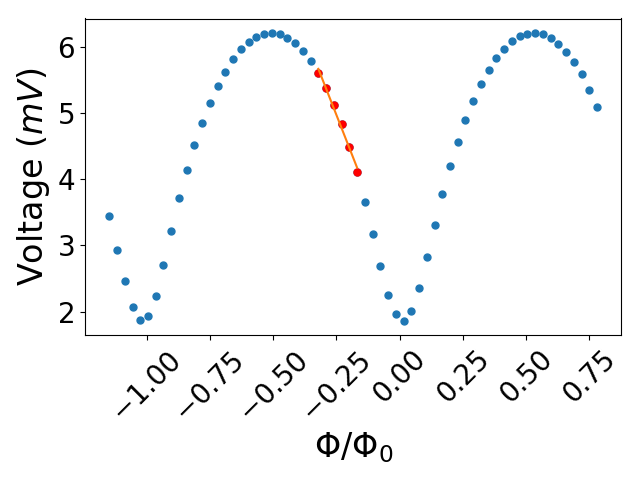
\includegraphics[height=2.5in]{figures/vphi_physical.png}
\caption{\ac{SQUID} voltage versus flux curve. The operating regime is highlighted (red) and fit to a line (orange) to get the \ac{SQUID} transimpedance.
\label{fig:squid_transimpedance} }
\end{center}
\end{figure}

The \ac{SQUID} noise could be measured, as was done in \ac{EBEX}, on a \ac{SQUID} not attached to a comb of bolometers (typically because of an open on one end of the microstrip) or it could be measured, as was done in \ac{ETC}, on a \ac{SQUID} with bolometers attached, but demodulating away from their resonant frequencies. 
Demodulating on-resonance gives a measure of the (4~K) bolometer Johnson noise in addition to the \ac{SQUID} noise.  



\begin{figure}[ht!]
\begin{center}
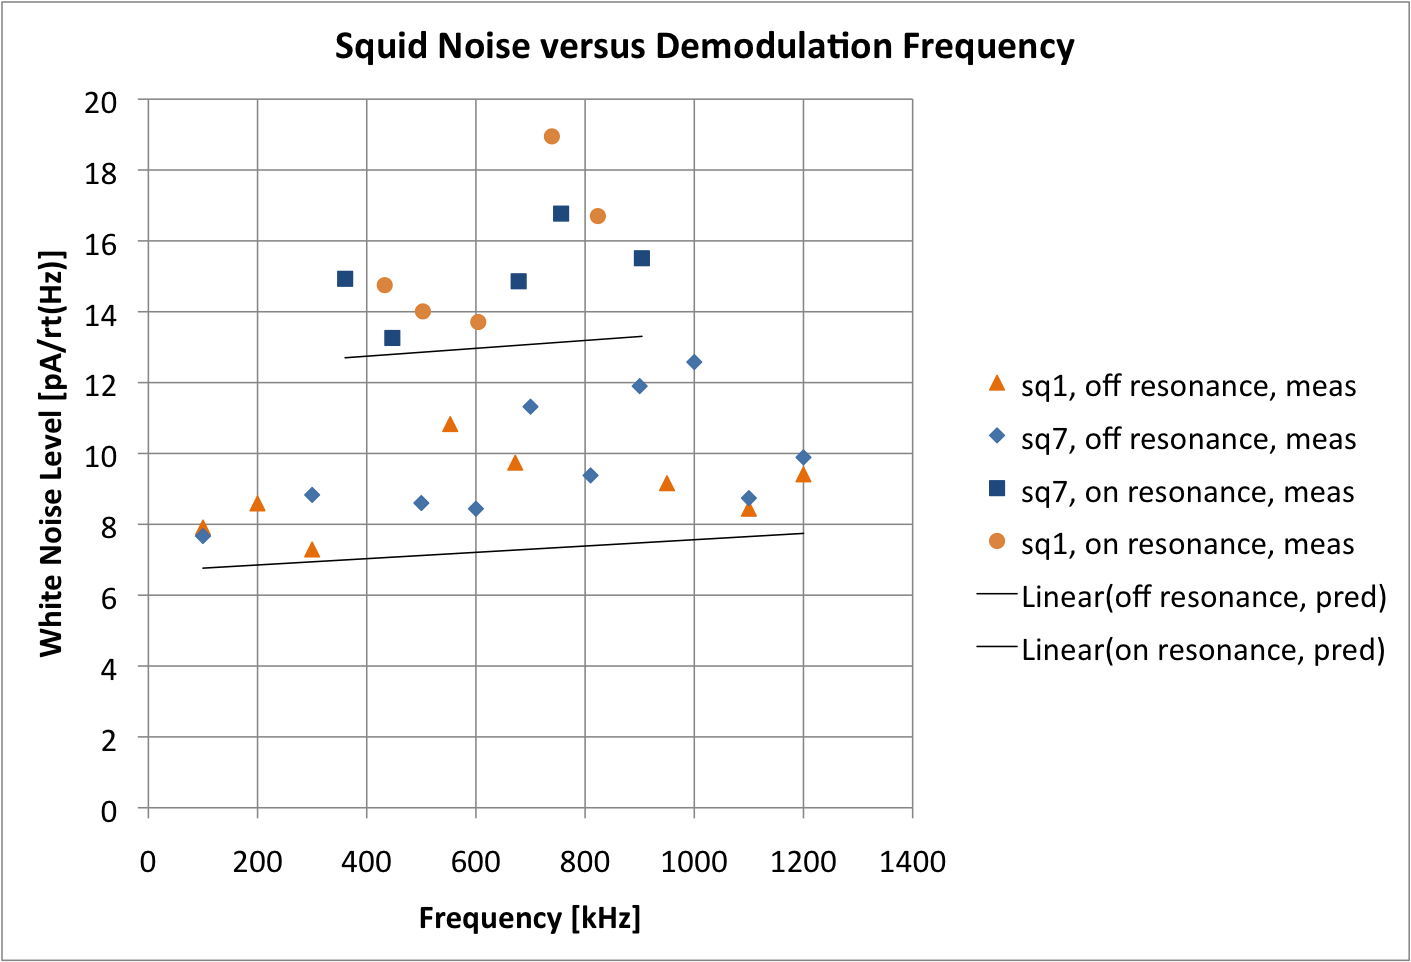
\includegraphics[height=2.5in]{figures/squidnoise_temp}
\caption{\ac{SQUID} noise in \ac{ETC} as function of demodulation frequency. At detector demodulation frequencies, the Johnson noise term of the bolometer roughly doubles the noise.
\label{fig:dark_squid_noise} }
\end{center}
\end{figure}



%%%%%%%%%%%%%%%%%%%%%%%%%%%%%%%%%%%%%%%%%%%%%%%%%%%%%%%%%%%%%%%%%%%%%%%%%%%%%}}}
